% !TeX root = ../main.tex

Dato il processo di sviluppo delle applicazioni mobile individuato nel capitolo \ref{ch:ch3} e definiti gli strumenti e task necessari, si descrive in questo capitolo come è stato automatizzato il processo adottando le moderne tecniche di integrazione continua e rilascio continuo al fine di fornire un modello di processo di sviluppo ai vari reparti aziendali che si occupano di applicazioni mobile.\\
Per la progettazione della pipeline è stato utilizzato il progetto base generato tramite il plugin Gradle KMM con lo scopo di mantenere il focus solamente sul processo e non sul prodotto. Tale progetto fornisce una applicazione essenziale sviluppata tramite KMM, comprensiva di modulo condiviso e moduli specifici sia Android che iOS.

\section{Continuous Integration}

\subsection{Build}
% cache android sdk, gradle e kotlin (https://kotlinlang.org/docs/native-improving-compilation-time.html#general-recommendations)
Tipicamente la fase iniziale della integrazione continua consiste nella verifica della corretta compilazione del codice sorgente. La compilazione rappresenta un vincolo essenziale per tutte le successive fasi e per questo è definita come fase bloccante: in caso di compilazione fallita la pipeline termina senza procedere con le fasi successive.\\
La fase di build definita svolge quindi il compito di validare la compilazione del codice condiviso (Kotlin) e del codice specifico Android (Kotlin) e iOS (Swift). 

\subsection{Testing}
Dopo aver verificato la corretta compilazione del codice la fase successiva è quella di test. In questa fase vengono eseguiti tutti gli unit test definiti, anche in questo caso sia per il codice condiviso che per il codice specifico Android e iOS.

\subsection{Analysis}
In questa sezione si descrivono le tecniche di analisi adottate e come queste sono state integrate nel processo di sviluppo sia per il codice sviluppato che per le dipendenze del sistema. Queste tecniche di analisi si distinguono rispettivamente in:
\begin{itemize}
    \item \textit{Static Application Security Testing} (SAST) - Analisi white-box della applicazione al fine di individuare vulnerabilità, code smell e bug.
    \item \textit{Software Composition Analysis} (SCA) - Analisi delle dipendenze di progetto con lo scopo di individuare vulnerabilità pubbliche (CVE)\footnote{Common Vulnerability and Exposure} associate ad esse.
\end{itemize}
In entrambe le tipologie di analisi è fondamentale ottenere come risultato uno o più report della scansione, in grado di descrivere in modo dettagliato eventuali "findings" trovati, ovvero l'insieme delle entità restituite dalla analisi/ricerca. I report vengono prodotti tipicamente sia in formati human-readable (es. pagina HTML) che machine-readable (es. JSON, XML, ...) per poter essere utilizzati da applicazioni terze come ad esempio servizi per centralizzare la consultazione di report eterogenei (\textit{Vulnerability Management System}).

\begin{figure}[H]
\centering
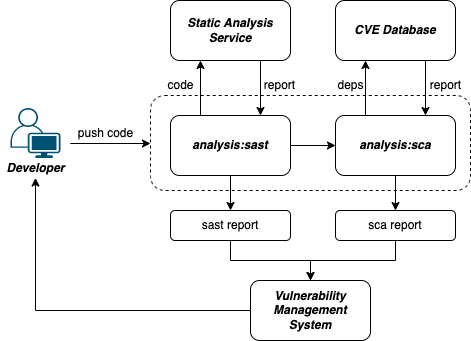
\includegraphics[width=0.7\textwidth]{img/tesi-12-sastsca.drawio.png}
\caption{Esempio tipico di integrazione della analisi statica e delle dipendenze nel processo di sviluppo automatizzato}
\end{figure}

Nel contesto aziendale Maggioli questi servizi sono messi a disposizione di tutti i team di sviluppo e mantenuti dalle figure responsabili della sicurezza informatica. Nello specifico i servizi aziendali disponibili sono:
\begin{itemize}
    \item \textit{SonarQube}\footnote{\url{https://github.com/SonarSource/sonarqube}} - Piattaforma open-source per effettuare analisi statica del codice.
    \item \textit{DefectDojo}\footnote{\url{https://github.com/DefectDojo}} - Piattaforma open-source per la gestione centralizzata delle vulnerabilità.
\end{itemize}

\subsubsection{Composizione Software}
Con composizione software si intende l'insieme di codice sviluppato da terze parti che viene incluso all'interno della applicazione, tipicamente sotto forma di import di librerie, dette dipendenze. Queste dipendenze includono a loro volta altre dipendenze e potrebbero introdurre vulnerabilità alla applicazione che le utilizza. \\
Per questo motivo è necessario analizzare le dipendenze al fine di individuare le vulnerabilità che esse introducono per essere tempestivi nel loro aggiornamento non appena vengono rilasciate delle patch di sicurezza. Il tool adottato per effettuare questa tipologia di analisi è \textit{Dependency Check}\footnote{\url{https://github.com/jeremylong/DependencyCheck}}, un tool open-source rilasciato e mantenuto da OWASP sia nella forma di plugin Gradle che come eseguibile e immagine Docker.

\begin{listing}[H]
\inputminted{kotlin}{code/4-depcheckplugin}
\caption{Configurazione plugin Gradle DependencyCheck per il modulo Android}
\end{listing}

\begin{listing}[H]
\inputminted{yaml}{code/4-depcheckjob}
\caption{Pipeline job dedicato alla analisi delle dipendenze della applicazione Android tramite l'utilizzo del plugin Gradle DependencyCheck}
\end{listing}

\subsubsection{Analisi Statica}
La fase di analisi statica viene eseguita per il codice condiviso e per il codice specifico considerando i tre moduli separatamente. I tool individuati e integrati nella fase di analisi statica del codice sono i seguenti:
\begin{itemize}
    \item \textit{Android Lint} (android, condiviso) - Tool per l'analisi statica di applicazioni Android, disponibile via CLI e via plugin Gradle (a partire dalla versione 16 ADT\footnote{Android Development Tools}).
    \item \textit{Detekt} (android, condiviso) - Tool per l' analisi statica del codice, specifico per il linguaggio di programmazione Kotlin, disponibile via CLI e via plugin Gradle.
    \item \textit{SonarQube} (android, condiviso, ios) - Client tool per l'interazione con il server SonarQube, disponibile via CLI e via plugin Gradle.
\end{itemize}

\begin{listing}[H]
\inputminted{yaml}{code/4-sastjob}
\caption{Pipeline job dedicato alla analisi statica del codice specifico Android}
\end{listing}

Data la funzionalità di gestione delle vulnerabilità fornita dallo stesso SonarQube e la possibilità di integrare tutte le tipologie di report prodotte sia nella fase di analisi delle dipendenze che nella fase di analisi statica del codice, si è deciso di non introdurre nel sistema l'utilizzo dei servizi forniti dalla installazione aziendale di DefectDojo.\\
Per le fasi di analisi, sia statica che dinamica, i tool hanno bisogno solo dei sorgenti e dei file di configurazione. Questo comporta il vantaggio di non dover compilare nessun file, scaricare nessun sdk, ... . Per questo motivo, dove possibile, è stata utilizzata l'immagine Docker del relativo tool come immagine per il job della pipeline.\\
Il client SonarQube utilizzato è stato dunque configurato, per poter considerare i report prodotti nelle altre fasi di analisi, agendo sui file \textit{build.gradle.kts} degli specifici moduli:
\begin{listing}[H]
\inputminted{kotlin}{code/4-sonarplugin}
\caption{Configurazione client SonarQube per il modulo condiviso (Shared)}
\end{listing}
\begin{figure}[H]
\centering
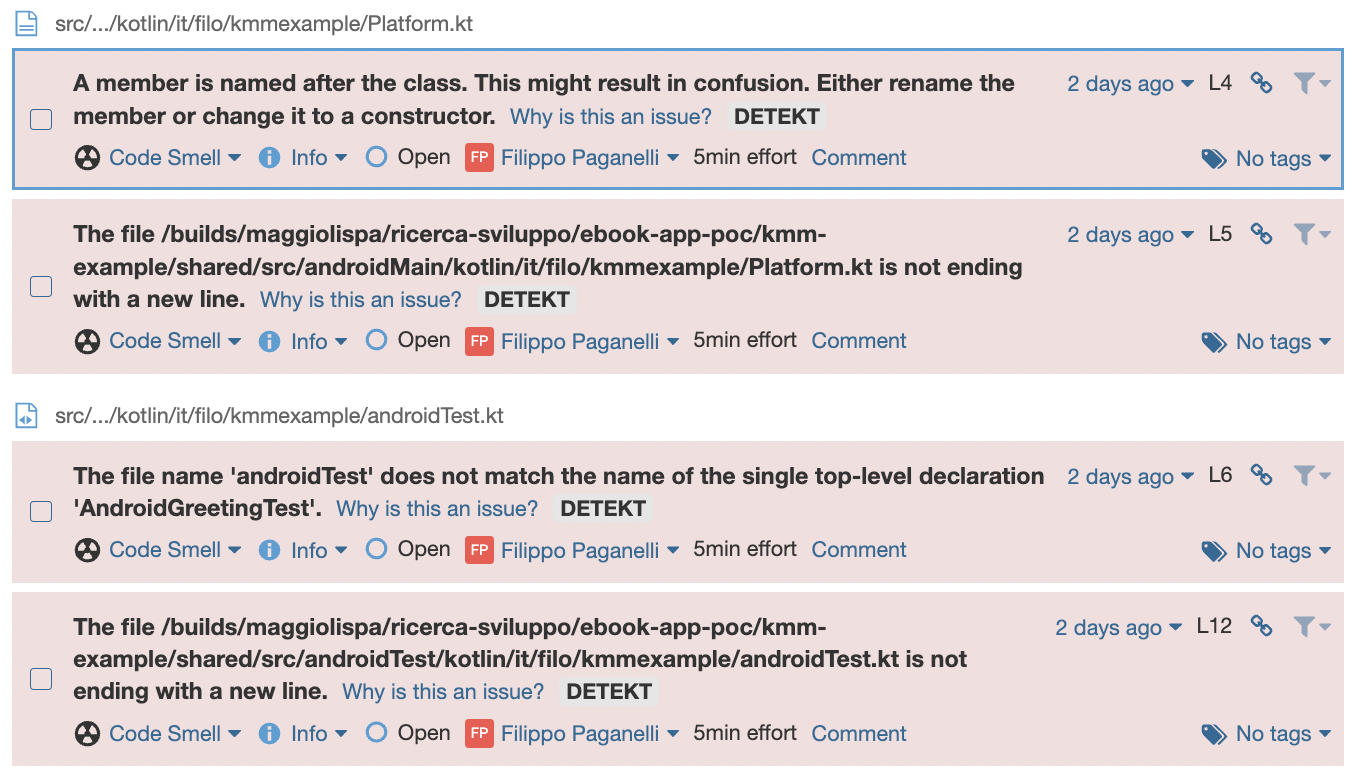
\includegraphics[width=1\textwidth]{img/Screenshot 2022-06-19 at 15.33.37.png}
\caption{Screenshot SonarQube Web UI - Esempio analisi modulo condiviso}
\end{figure}
\begin{figure}[H]
\centering
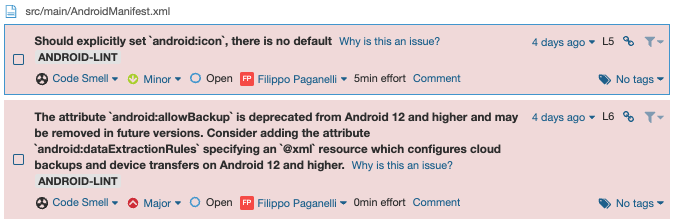
\includegraphics[width=1\textwidth]{img/Screenshot 2022-06-21 at 09.58.58.png}
\caption{Screenshot SonarQube Web UI - Esempio analisi modulo android}
\end{figure}
\subsection{Package}
Definiti i passi di compilazione, testing e analisi del codice la parte di integrazione continua termina con la pacchettizzazione dell'applicazione. In questa fase del processo il codice sorgente viene impacchettato in modo automatico nei formati richiesti dalle piattaforme target, ovvero \textit{.apk}\footnote{Android Package} per Android e \textit{.ipa}\footnote{iOS App Store Package} per iOS.

\section{Continuous Delivery}

\subsection{Fastlane}
Uno fra i tool open-source più diffusi a supporto della automazione dello sviluppo di applicazioni mobile, sia Android che iOS, è Fastlane\footnote{\url{https://github.com/fastlane/fastlane}}. L'impiego principale di questo tool è nella automazione della fase di rilascio della applicazione, sia in beta che in produzione, grazie alla gestione di tutti quei task necessari ma dispendiosi in termini di tempo come: generazione degli screenshot, firma digitale del codice (\textit{Code Signing}), ... .\\
Si fa uso dei seguenti concetti per configurare fastlane nell'apposito file di configurazione (\textit{Fastfile}) e con sintassi Ruby:
\begin{itemize}
    \item \textit{Action} - Elaborazioni pre-definite e configurabili tramite passaggio di parametri.
    \item \textit{Lane} - Insieme di action definito dall'utente per descrivere elaborazioni più complesse.
\end{itemize}

\begin{listing}[H]
\inputminted{ruby}{code/4-fastlane}
\caption{Esempio Fastlane: lane per il rilascio in versione beta di applicazioni iOS}
\end{listing}

\subsection{Alpha Release}
% rilascio sul package registry gitlab, versionamento con l hash della commit ad ogni modifica sul branch dev. ogni versione che dal branch dev viene portata sul branch test diventa una beta release (pubblicata su testflight e google play console) e ogni versione che da test viene portata su main diventa una prod release (pubblicata su app store e google play).

\subsection{Beta Release}

\subsection{Production Release}

\section{Continuous Monitoring}
\subsection{Monitoring}
\subsection{Analytics}

\section{Infrastruttura}
% descrivere l'infrastruttura necessaria a supporto della cicd: runners, nexus, sonarqube, defectdojo, cluster, ecc

\section{Templating}
% definire la cicd in template in un progetto a parte in modo che possano essere importati nel PoC (ed essere usati da altri in futuro)
% dire come gitlab permette di farlo, quali sono i meccanismi ecc ecc
% lo stesso risultato dei gitlab template può essere ottenuto distribuendo delle github action
